\documentclass[fr]{../../../eplsummary}

\usepackage{../../../eplcode}
\usepackage{../../../eplunits}
\usepackage{tikz}
%\usepackage{pgf-umlcd}
\usepackage{pgf-umlsd}
\usepgflibrary{arrows} % for pgf-umlsd

\usepackage{graphicx}
\usepackage{verbatim}

\lstset{language=SQL, morekeywords={DATABASE,ESCAPE,IS,REAL,REFERENCES,TEXT}}

\hypertitle{Conception orient\'ee objet et gestion de bases de donn\'ees}
{4}{SINF}{1225}
{Beno\^it Legat\and Benjamin de Wergifosse}
{Kim Mens}

\part{Gérer une base de données avec le langage SQL}
Une base de données permet de stocker des informations de manières structurées
et facilement accessible.
Les données y sont organisées en tables selon un thème,
une \strong{collection d'entités} (ex. Clients, Réservations,...).
Il faut cependant veiller à créer ces tables de manières intelligentes:
il faut
\begin{itemize}
  \item éviter les données redondantes
    (que l'on peut trouver grâce à d'autres),
  \item veiller à ce qu'on puisse faire le lien entre les différentes
    tables grâce à des références (ID),
  \item éviter les redondances au sein d'une même table
    ($\Rightarrow$ on split la table).
\end{itemize}

Dans une table,
si une colonne est constituée de valeurs uniques,
on dit qu'elle est un \strong{identifiant} de la table,
elle constitue une \strong{clé primaire}.
Si une colonne contient des informations (un ID par exemple) qui permettent
de récupérer des informations associées dans une autre table,
on nomme la colonne de \strong{clé étrangère}.

Une base de données se gère grâce au langage SQL
qui possède une syntaxe particulière.
Nous allons voir les principales requêtes permettant d'accéder aux données,
de les modifier et d'en ajouter.
D'autres parts, un logiciel,
que l'on nomme \strong{système de gestion de bases de données},
permet la gestion sur disque des tables.
Il assure la sécurité, la confidentialité,
l'archivage et la restauration des informations.
Les requêtes SQL sont envoyées au programme qui les comprends et
va chercher sur le disque les informations relatives aux requêtes.
On utilisera SQLite,
un SGBD léger et efficace utilisé par les applications d'Android et iOS.

En SQLite, les types possibles sont

\begin{itemize}
  \item \lstinline|INTEGER|, c'est un entier signé sur 1, 2, 3, 4, 6, ou 8 bytes
    en fonction de sa taille;
  \item \lstinline|REAL|, c'est un nombre à virgule flottante sur 8 bytes
    selon la norme IEEE;
  \item \lstinline|TEXT|, c'est un string, stocké en utilisant
    l'encodage de la base de donnée (UTF-8, UTF-16BE ou UTF-16LE);
  \item \lstinline|BLOB|, c'est un blob de donnée,
    stocké exactement comme tel, utile pour les images.
\end{itemize}
Il y a aussi le mot clef \lstinline|NULL| qui est l'équivalent
d'une valeur absente.

\section{Création, modification et suppression de tables}
On crée une table avec le mot clef \lstinline|CREATE TABLE|
Pour chaque colonne, il faut donner sont nom, son type
et des options supplémentaires
\begin{itemize}
  \item \lstinline|NOT NULL| indique qu'une entrée doit toujours compléter
    cette colonne;
  \item \lstinline|UNIQUE| indique qu'on ne peut pas avoir plusieurs
    entrées qui ont la même valeur pour cette colonne;
  \item \lstinline|PRIMARY KEY| indique ce c'est la clef primaire qu'on
    utiliser pour référencer les entrées.
    \lstinline|NOT NULL| et \lstinline|UNIQUE| sont implicite lorsqu'on a
    \lstinline|PRIMARY KEY|;
  \item \lstinline|REFERENCES| indique que les éléments de cette colonne
    font référence à des entrées d'une table.
\end{itemize}

Voici un exemple de table non-relationnelle, c'est à dire sans
\lstinline|REFERENCES|
\begin{lstlisting}
CREATE TABLE blades (
  id PRIMARY KEY,
  color TEXT NOT NULL,
  length REAL NOT NULL);
\end{lstlisting}
et en voici un avec relation
\begin{lstlisting}
CREATE TABLE jedis (
  name TEXT NOT NULL,
  blade_id INTEGER,
  PRIMARY KEY (name),
  FOREIGN KEY (blade_id) REFERENCES blade);
\end{lstlisting}
qui peut aussi être écrit
\begin{lstlisting}
CREATE TABLE jedis (
  name TEXT PRIMARY KEY,
  blade_id INTEGER NOT NULL REFERENCES blades);
\end{lstlisting}

On peut aussi ajouter une colonne à une table déjà créée
\begin{lstlisting}
ALTER TABLE jedis ADD COLUMN height REAL;
\end{lstlisting}
et supprimer une table
\begin{lstlisting}
DROP TABLE jedis;
\end{lstlisting}

\section{Sélection dans une base de donnée}
On peut sélectionner des entrées,
\begin{lstlisting}
SELECT LastName, FirstName FROM Persons
SELECT * FROM Persons
SELECT DISTINCT City FROM Persons
\end{lstlisting}

les filtrer selon des conditions
\begin{lstlisting}
SELECT column_name1, column_name2, ...  FROM table_name
WHERE column_name operator value
\end{lstlisting}
Dans le \lstinline|WHERE|,
on peut utiliser les opérateurs suivant
\begin{lstlisting}
Operator  Description
=         Equal
<>        Not equal
>         Greater than
<         Less than
>=        Greater than or equal
<=        Less than or equal
BETWEEN   Between an inclusive range
LIKE      Search for a pattern
IN        To specify multiple possible values for a column
/* Note: In some versions of SQL the <> operator
 * may be written as !=
 */
\end{lstlisting}

qui peuvent contenir les mots clefs \lstinline|AND| et \lstinline|OR|
\begin{lstlisting}
SELECT * FROM Persons WHERE FirstName='Jean'
                        AND (LastName='Dupond' OR LastName='Dupont')
\end{lstlisting}

et qui peuvent être ordonnés
\begin{lstlisting}
SELECT * FROM Persons ORDER BY LastName DESC
\end{lstlisting}
Dans cette requête \lstinline|DESC| indique qu'on
ordonne en ordre décroissant. L'ordre par défaut est
croissant (mot clé \lstinline|ASC|).

\subsection{Examples de requêtes}
L'aspect le plus intéressant de SQL sont les références.
On peut par exemple obtenir les jedis sans sabre laser
\begin{lstlisting}
SELECT name
FROM jedis
WHERE blade_id IS NULL; /* ATTENTION PAS blade_id = NULL */
\end{lstlisting}
ou le contraire
\begin{lstlisting}
SELECT name
FROM jedies
WHERE blade_id IS NOT NULL;
\end{lstlisting}
mais aussi le nom des jedis ayant un sabre laser rouge
\begin{lstlisting}
SELECT J.NAME
FROM JEDI J, LASER_BLADE LB
WHERE J.BLADE_ID = LB.ID
and LB.COLOR = 'red';
\end{lstlisting}
Cette commande peut aussi être écrite comme suit
\begin{lstlisting}
SELECT NAME
FROM JEDI
WHERE BLADE_ID in
(SELECT ID
FROM BLADE WHERE COLOR = 'red');
\end{lstlisting}
mais c'est moins efficace car la précédente est mieux optimisée par
les SGBD.

Pour éviter d'avoir des répétitions, on peut utiliser le mot clef
\lstinline|DISTINCT| qui vérifie que les $n$-uples en sortie sont tous
distincts.
C'est à dire qu'ils peuvent avoir certaines colonnes les mêmes mais pas toutes.
Par exemple, dans l'exemple suivant,
\begin{lstlisting}
SELECT DISTINCT b.color
FROM jedis j, blades b
WHERE j.height < 1.20 AND j.blade_id = b.id;
\end{lstlisting}
on sélectionne les couleurs de sabres lasers de jedis de moins
de \unit{1.2}{\meter}.

Il y a aussi le mot clef \lstinline|IN|,
\begin{lstlisting}
SELECT name
FROM jedis j, blades b
WHERE j.blade_id = b.id AND b.color IN ('red','blue','green');
\end{lstlisting}
\begin{lstlisting}
SELECT name
FROM jedis j
WHERE j.blade_id = b.id AND b.color NOT IN ('red','blue');
\end{lstlisting}
le mot clef \lstinline|BETWEEN|
\begin{lstlisting}
SELECT name
FROM jedis j
WHERE height BETWEEN 1 AND 2;
\end{lstlisting}
et le mot clef \lstinline|LIKE|
\begin{lstlisting}
SELECT name
FROM jedis
WHERE name LIKE 'Yo__'; /* Yoda */

SELECT name
FROM jedis
WHERE name LIKE '%Wan%'; /* 'Obi-Wan Kenobi', 'Obi-Wan', ... */
\end{lstlisting}
à qui on peut aussi définir un caractère d'échappement
avec \lstinline|ESCAPE|
\begin{lstlisting}
SELECT name
FROM jedis
WHERE name like '%!_% 100!% !!' ESCAPE '!';
/* 'super_jedi 100% cool !' */
\end{lstlisting}

On peut effectuer des calculs sur la sortie
\begin{lstlisting}
SELECT j.height + b.length
FROM jedis j, blades b;
\end{lstlisting}
et changer le nom des colonnes avec des alias
\begin{lstlisting}
SELECT name, j.height + b.length AS total_size
FROM jedis j, blades b;
\end{lstlisting}

\section{Modification des entrées}
\subsection{Insérer une nouvelle entrée}
La syntaxe est la suivante
\begin{lstlisting}
INSERT INTO table_name VALUES (value1, value2, value3,...)
INSERT INTO table_name (column1, column2, column3,...) VALUES (value1, value2, value3,...)
\end{lstlisting}

On peut complèter les colonnes dans l'ordre
\begin{lstlisting}
INSERT INTO jedis
values ('Anakin Skywalker',42,1);
\end{lstlisting}
mais ce n'est pas très lisible.
On peut donc être plus explicite et les remplir dans l'ordre que l'on veut
\begin{lstlisting}
INSERT INTO jedis (name,blade_id,height)
values ('Anakin Skywalker',1,42);
\end{lstlisting}

On peut aussi insérer dans une tables
des données obtenue par un \lstinline|SELECT|.
Supposons qu'on veule mettre dans une table le noms des jedis qui ont
rejoint le côté obscur
\begin{lstlisting}
INSERT INTO DARK_SIDE
SELECT j.name
FROM jedis j, blades b
WHERE j.blade_id = b.id AND b.color = 'red';
\end{lstlisting}

\subsection{Mettre à jour des entrées}
La syntaxe est la suivante
\begin{lstlisting}
UPDATE table_name SET column1=value1, column2=value2, ...
WHERE some_column=some_value AND some_column=some_value AND ...
\end{lstlisting}

On peut par exemple changer le nom et la couleur du sabre d'Anakin
Skywalker avec
\begin{lstlisting}
UPDATE jedis j, blades b
SET j.name = 'Dark Vador', b.color = 'red'
WHERE j.name = 'Anakin Skywalker' AND j.blade_id = b.id;
\end{lstlisting}

\subsection{Supprimer des entrées}
La syntaxe est la suivante
\begin{lstlisting}
DELETE FROM table_name
WHERE some_column=some_value AND some_column=some_value AND ...
\end{lstlisting}

On peut par exemple supprimer ``Qui-Gon''
\begin{lstlisting}
DELETE FROM jedis
WHERE name = 'Qui-Gon';
\end{lstlisting}

Ou supprimer tous les jedis du dark side
\begin{lstlisting}
DELETE j FROM jedis j, blades b
WHERE j.blade_id = b.id AND b.color = 'red';
\end{lstlisting}

Ou supprimer ceux qui n'ont plus de sabre laser
\begin{lstlisting}
DELETE FROM jedis
WHERE j.blade_id IS NULL;
\end{lstlisting}

\part{Modélisation de données ORM et mapping relationnel}
Dans le processus de développement d'une application orientée objet,
il est important de bien penser son application avant de se
pencher sur l'implémentation de son code source.
Ainsi diverses étapes d'analyse du problème sont requises.
La modélisation de données selon l'approche
ORM (Object-Role Modeling) est en la première.

Dans un premier temps,
il est important de définir \strong{l'univers de discours} (UoD).
Celui-ci, en une phrase, définit le domaine de l'application.

\section{Le modèle relationnel et les relations $n$-aires}
On cherche à définir les relations qui existent.
Ces relations définiront les tables SQL qui seront créées.
À une relation correspondra une table.
Le \strong{schéma de la relation} reprend les noms des colonnes de
la table qui lui correspondra.
Par exemple, on pourrait imaginer le schéma de la relation
\lstinline|CLIENT| suivant
\begin{lstlisting}
CLIENT(ID, SORTE, NOM, PRENOM, ADRESSE)
\end{lstlisting}
Dans le modèle relationnelle, on n'utilise pas la notation positionnelle.
Dès lors, un mutliplet \lstinline|CLIENT| sera toujours
un ensemble de couple \lstinline$(TITRE, valeur)$.
On pourrait imaginer la \strong{relation} basée sur
le schéma ci-dessus comme étant l'ensemble de multiplets suivant:
\begin{lstlisting}
{
  {(ID,459), (SORTE,externe), (NOM,Horner), (PRENOM,Yvette), (ADRESSE,"7, impasse des capucines, Wavre")},
  {(ID,3124), (SORTE,interne), (NOM,Dupont), (PRENOM,Jules), (ADRESSE,"3, rue des combattants, La Hulpe")},
  ...,
  {(ID,6789), (SORTE,externe), (NOM,Gave), (PRENOM,Jean), (ADRESSE,"32, avenue des allies, Tournai")},
  {(ID,6947), (SORTE,interne), (NOM,Durant), (PRENOM,Alfred), (ADRESSE,"17, allee des saules, Plancenoit")}
}
\end{lstlisting}
Le transfert de cette relation vers une table est immédiat.
La base de données est donc un ensemble de table basées
sur un ensemble de relations $n$-aires.
La \strong{schéma de la base de données} n'est
autre que l'ensemble des schémas des différentes relations.

\section{L'Object-Role Modeling}
Fortement basé sur le modèle relationnel simple présenté ci-dessus,
l'ORM en est une amélioration qui permet d'éviter les redondances,
qui est plus conforme au monde réel et plus intuitif et facile à comprendre.
Cette approche tient compte du fait qu'une base de données
peut être vue comme un ensemble de \strong{faits} (les données)
et de \strong{règles} (liens entre les faits) s'articulant autour
d'un \strong{univers de discours}.
Ainsi, 3 étapes permettent la modélisation ORM.

\subsection{Les faits élémentaires}
Premièrement,
il faut, en se basant sur des exemples de données,
établir une liste de \strong{faits élémentaires}.
Un fait élémentaire est une assertion simple et atomique
sur l'univers de discours.
Un fait élémentaire fait intervenir des \strong{objets} et leur \strong{rôle}.
Il y a deux types d'objets:
les VALEURS et les entités (= ensemble TYPE-MODE-VALEUR).
Exemples:
\begin{itemize}
  \item Client-nom-``UCL''
  \item Facture-numéro-0254968065768
  \item Montant-euro-275
\end{itemize}

Selon qu'un fait élémentaire fait intervenir plus ou moins d'objets
on dira qu'elle est \strong{unaire} (1),
\strong{binaire} (2) ou \strong{$n$-aire} ($n$).
Voici quelques exemples de faits élémentaires :
\begin{itemize}
  \item Destination-numéro-0475151230 \emph{est gratuite};
  \item Opérateur-nom-``Proximus'' \emph{a} Préfixe-numéro-0478;
  \item Communication-numéro-11 \emph{a} Durée-minutes-``$1:38$'';
  \item Facture-numéro-0648979136879 \emph{coûte} Montant-euro-289;
  \item Etudiant-noma-54511100 \emph{a obtenu} Cote-chiffre-18
    \emph{pour} Cours-code-``LSINF1125'';
  \item Jedi-nom-Yoda \emph{mesure} Taille-mètre-\np{0.66}.
\end{itemize}
Il est à noter qu'un fait élémentaire ne peut pas être divisé et
qu'il n'utilise aucun connecteurs logiques (et, ou, non, si).

\subsection{Dessiner les types de faits + population}
Le but de cette étape est de créer un \strong{schéma conceptuel}
(voir figure~\ref{schema_conceptuel}).
Pour cela il faut identifier les TYPES d'objets,
leur MODE (type de valeur)
et la relation $n$-aire s'y rapportant.
L'exemple n'illustre que des relations binaires mais l'extension
à la relation ternaire est immédiate
(ajout d'une boite sur la ligne de relation).
\begin{figure}[h]
  \centering
  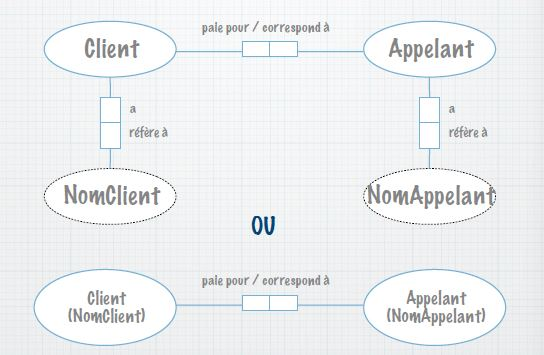
\includegraphics[scale=0.7]{schema_conceptuel.jpg}
  \caption{Exemple d'un schéma conceptuel}
  \label{schema_conceptuel}
\end{figure}
Une fois le schéma créé,
il faut lui ajouter une population exemple pour
s'assurer de l'exactitude de celui-ci.

\subsection{Les contraintes}
Le schéma est encore loin d'être terminé,
il faut maintenant lui ajouter les \strong{contraintes d'unicité}
(voir figure~\ref{contraintes}).
Ces contraintes permettent de déterminer si une valeur peut se retrouver
une ou plusieurs fois dans une même colonne.
Une bonne population exemple facilite le choix des contraintes.
L'exemple donné illustre les contraintes pour la relation binaire mais
l'extension pour le cas ternaire est immédiate.
Dans ce cas,
il est évident qu'il n'y aura jamais de contrainte ``simple''
auquel cas on pourrait diviser la relation en deux autres binaires.
\begin{figure}[h]
  \centering
  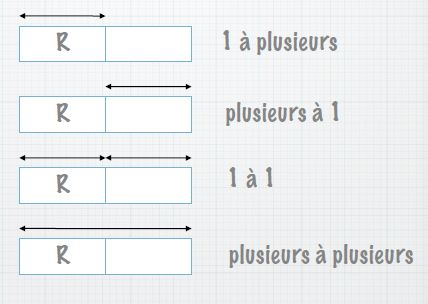
\includegraphics[scale=0.8]{contraintes.jpg}
  \caption{Contraintes possibles pour une relation binaire}
  \label{contraintes}
\end{figure}
La figure~\ref{fig:schema_conceptuel_complet} illustre un usage où on
stipule qu'un étudiant a au plus un nom et au plus une classe.

Il faut également ajouter les contraintes de \strong{rôles obligatoires}.
En effet il se peut que l'on veille stipuler que la relation
liant deux objets doit être obligatoire.
Pour ce faire, on place un point sur la ligne de relation du côté
de l'entité qui doit apparaitre au moins une fois dans les exemples.
La figure~\ref{fig:schema_conceptuel_complet} en illustre un usage où
on stipule qu'il est obligatoire pour un étudiant d'avoir
au moins un nom et au moins une classe.

Une autre contrainte à ajouter sur le schéma conceptuel est celle
d'\strong{unicité externe}.
En effet, il se peut qu'un objet ayant plusieurs relations soit déterminé
de manière uniquement par la combinaison de plusieurs objets avec lesquels
il est en relation.
Par exemple un fichier qui serait en relation avec un dossier et un nom de
fichier est déterminé
de manière unique par le couple (dossier, nom de fichier).
La figure~\ref{fig:schema_conceptuel_complet} illustre un autre exemple
où on stipule qu'il n'y a pas deux élèves avec
le même nom dans la même classe.
On peut donc référencer un élève par son nom et sa classe.

La dernière contrainte possible est la \strong{contrainte de sous-ensemble}.
Cette contrainte stipule qu'une relation ne peut exister que
si une autre (qui n'est donc pas obligatoire) est satisfaite.
Elle se dessine comme une flèche en pointillé d'une boite
à celle obligatoire (un peu comme l'unicité externe).

\begin{figure}[h]
  \centering
  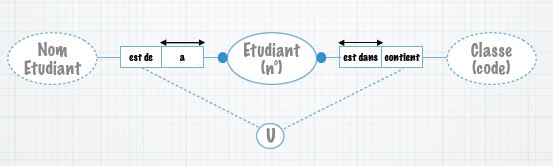
\includegraphics[scale=0.8]{schema_conceptuel_complet}
  \caption{Exemple complet d'un schéma conceptuel}
  \label{fig:schema_conceptuel_complet}
\end{figure}

\section{Schéma relationnel}
Après avoir transformé les relations $n$-aires du modèle relationnel
en schéma conceptuel ORM,
il est maintenant temps de transformer le schéma conceptuel
ORM et \strong{schéma relationnel}.

Le principe consiste à choisir un objet clé du schéma conceptuel
et de le transcrire sous forme de tableau.
Dans ce tableau doit se retrouver toutes les contraintes du schéma conceptuel.
Ainsi,
\begin{itemize}
  \item les colonnes sont soulignées si elles sont uniques;
  \item les colonnes sont soulignées par la même lignes quand elles
    font partie d'une unicité externe commune;
  \item les colonnes sont mises entre crochet si elles ne sont optionnelles;
  \item les deux clés primaires de tableaux différents
    (si toutefois les données sont dans deux tableaux différents)
    sont reliés par une flèche pour une
    contrainte de sous-ensemble.
\end{itemize}

La clef primaire doit exister et être unique, c'est donc
\begin{itemize}
  \item soit une colonnes obligatoire et unique;
  \item soit plusieurs colonnes obligatoire avec une unicité externe.
\end{itemize}
Dans le premier cas, la colonne correspondante est soulignée deux fois.
Dans le deuxième, les colonnes correspondantes sont soulignées deux fois
par les même lignes.

La clef primaire consitue la \strong{règle d'intégrité des entités}.
D'autres parts, lors d'une contrainte de sous-ensemble,
la flèche venant de la clé étrangère doit pointer vers une clé primaire.
Il s'agit de la \strong{règle d'intégrité référentielle}.

La figure~\ref{schema_relationnel} illustre un exemple de schéma relationnel
avec les différentes contraintes représentées.
\begin{figure}[h]
  \centering
  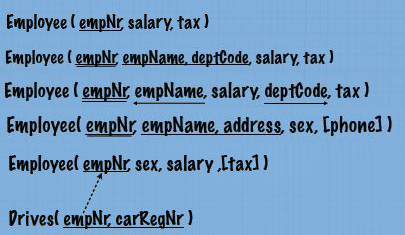
\includegraphics[scale=0.9]{schema_relationnel.jpg}
  \caption{Exemple schéma relationnel}
  \label{schema_relationnel}
\end{figure}

La figure~\ref{conceptuel_to_relationnel} illustre un exemple un peu plus
élaboré du passage d'un schéma conceptuel vers un schéma relationnel.
\begin{figure}[ht]
  \centering
  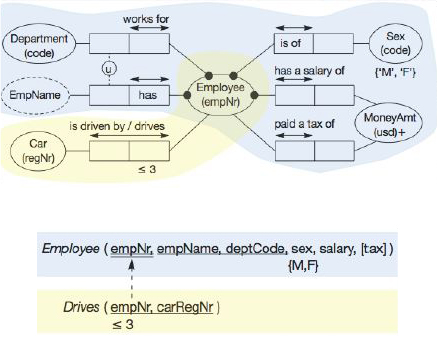
\includegraphics[scale=1]{conceptuel_to_relationnel.jpg}
  \caption{Exemple du passage d'un schéma conceptuel vers un schéma relationnel}
  \label{conceptuel_to_relationnel}
\end{figure}


\section{Le Relational Mapping}
Cette dernière étape permet, à partir du schéma relationnel,
de construire la base de données SQL.
La règle est relativement simple, deux règles sont à respecter:
\begin{enumerate}
  \item Les types de faits avec contraintes d'unicité composées
    sont mis dans des tableaux séparés.
  \item Tous les types de faits avec des rôles fonctionnels (unicité simple)
    liés à un même type d'objet sont regroupé dans un même tableau
    avec comme clé l'identifiant de ce type d'objet.
\end{enumerate}

\part{Processus de développement}
Dans la section précédente, nous avons vu comment modéliser,
de manière efficace, les données qui seront utilisées par l'application.
Cette modélisation par l'approche ORM nous a permis d'obtenir une solide
base de données SQL.
À présent, il est temps de se pencher sur la question de l'implémentation.
Comment va-t-on implémenter notre application, que doit-elle pouvoir faire,...
Il est important de suivre un \strong{processus de développement}
rigoureux qui nous permettra d'implémenter une bonne application.
Observons différents processus possibles.

\begin{figure}[h]
  \centering
  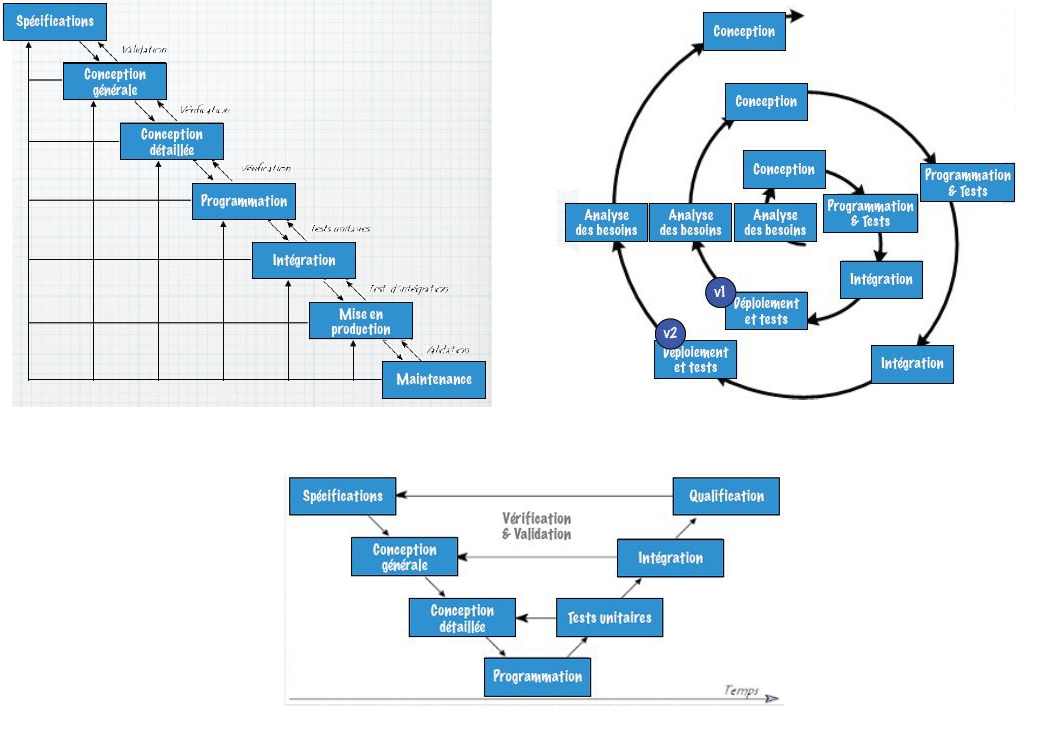
\includegraphics[scale=0.58]{processus_developpement_example.jpg}
  \caption{Différents processus de développement possibles}
  \label{processus_developpement_example}
\end{figure}

La figure~\ref{processus_developpement_example}
montre 3 exemples de processus de développement qui existent.

En haut à gauche, on retrouve le \strong{modèle en cascade avec retour}.
Celui-ci tient compte du fait que l'on ne peut bâtir
un toit sans avoir les fondations.
Ainsi une fois l'étape une terminée,
on passe à la suivante et ainsi de suite en cascade.
Cependant un retour à l'une des phases précédentes est possible mais
la modification de celle-ci à un important coût sur le reste du développement,
ce qui rend cette approche peu pratique et non efficace.

Au milieu, on observe le \strong{cycle en V}.
Il s'agit d'une amélioration du modèle précédant
car il permet de limiter le retour aux étapes précédentes.

À droite, le \strong{modèle en spirale} reprend l'idée du cycle en V mais
recommence à chaque boucle tout le processus de manière à obtenir
des versions successives de plus en plus complètes.

Le meilleur modèle pour la conception orientée objet est
typiquement \strong{itératif et incrémental}.
Ainsi la figure~\ref{processus_developpement_choisi}
illustre les différentes étapes de ce modèle.
On retrouve ainsi la phase d'INCEPTION où l'on
décrit l'objectif et l'ampleur du projet.
Ensuite, lors de l'ELABORATION, on imagine comment on va réaliser le système.
La phase de FABRICATION, décrite ci-dessous, est itérative et incrémental.
Pour finir la phase de TRANSITION permet d'optimiser le logiciel
en le testant et améliorant les performances.
\begin{figure}[h]
  \centering
  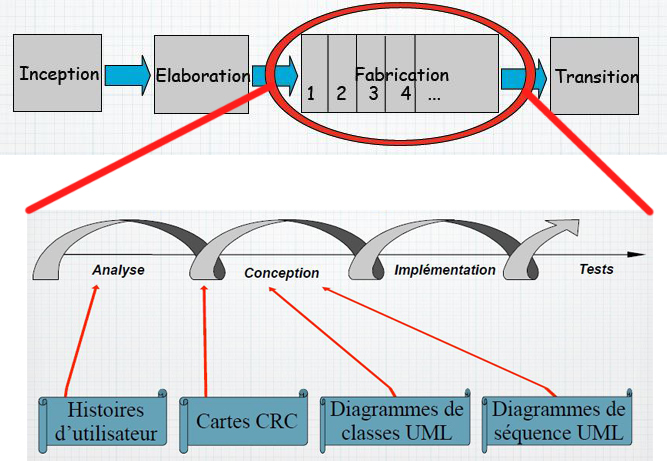
\includegraphics[scale=0.65]{processus_developpement_choisi.jpg}
  \caption{Processus itératif et incrémental choisi}
  \label{processus_developpement_choisi}
\end{figure}

La phase de FABRICATION reprend différentes itérations tels que
\begin{itemize}
  \item l'analyse par le biais d'histoires d'utilisateurs,
  \item la transition analyse-conception via les cartes CRC,
  \item la conception grâce aux diagrammes de classes UML et
  \item diagrammes de séquences UML
  \item pour arriver à l'implémentation.
\end{itemize}

\section{Les histoires utilisateur}
Dans un premier temps,
il faut définir ce qu'on appelle les
\strong{histoires utilisateur} (user stories).
Celles-ci définissent les besoins,
les exigences de l'application.
On distinguera les besoins fonctionnels (fonctionnalités de l'application) et
les besoins non-fonctionnels (fiabilité, performance).
Généralement une histoire est une courte description d'un besoin
dans un langage de haut niveau compréhensible par tous.
Chaque histoire suit le schéma basique suivant :
\begin{quote}
  \emph{En tant que ``rôle'',
  \\je veux ``action'',
  \\afin d' ``atteindre un objectif''.}
\end{quote}
Il est important de ne pas trop détailler les histoires
et de les écrire à la voix active.
Aussi, pour le programmeur,
on peut ajouter le temps que l'on pense qu'il faudra pour
implémenter cette fonctionnalité à notre application.
Typiquement une histoire prend 2 jours à implémenter.
Voici deux exemples d'histoires utilisateurs :
\begin{itemize}
  \item \emph{En tant que} nouvel utilisateur de l'application,\\
    \emph{afin d'}adapter l'information fournie par l'application à mon âge,
    ma langue préférée et mes centres d'intérêts,\\
    \emph{je veux} pouvoir encoder un profil
    personnalisé lors du premier démarrage de l'application.
  \item	\emph{Afin de} pouvoir modifier mon profil personnalisé,\\
    \emph{en tant qu'}utilisateur connu par l'application,\\
    \emph{je veux} pouvoir changer mon profil personnalisé à n'importe
    quel moment via un menu dédié et,
    si mon utilisateur est actif,
    les informations fournies par l'application s'adapteront immédiatement
    à mon nouveau profil.
\end{itemize}

Le mot clé ``INVEST'' caractérise une bonne histoire utilisateur :
\begin{description}
  \item[Indépendant] Il faut rendre chaque histoire
    le plus indépendante les unes des autres.
  \item[Négociable] Une histoire n'est pas fixée une fois pour
    toute, la conversation avec le client peut amener à la modifier.
  \item[Valuable] Chaque histoire a
    sa propre valeur en fonction de son importance.
  \item[Estimable] À chaque histoire est associé un
    ``coût'' d'implémentation.
  \item[Small]Une histoire ne doit pas
    être trop grande (ni trop petite) sinon elle peut être divisée.
  \item[Testable]On peut tester si une histoire est réalisée ou pas.
\end{description}

\section{Les cartes CRC}
Les cartes CRC, pour \strong{classes, responsabilités et collaborations},
permettent, comme leur nom l'indique,
d'obtenir une première idée des objets et classes qu'il faudra implémenter.
Ces classes auront certaines responsabilités en fonction des collaborations
qu'elles auront avec d'autres classes.

Propice pour le travaille en groupe,
cette méthode use de l'utilisation de petites cartes
permettant une représentation visuelle facile.
Chaque carte correspond à une classe,
contient une brève description de celle-ci,
ses responsabilités et collaborations (voir tableau~\ref{tab:crc}).

\begin{table}[h]
  \centering
  \begin{tabular}{|p{0.4\textwidth}|p{0.4\textwidth}|}
    \hline
    \multicolumn{2}{|l|}{\strong{Classe}: nom de la classe}\\
    \hline
    \multicolumn{2}{|l|}{\strong{Description}: courte description de la classe}\\
    \hline
    \strong{Responsabilités} & \strong{Collaborations}\\
    liste des différentes responsabilités de cette classe &
    classes avec lesquelles cette classe collabore pour réaliser
    ses différents responsabilités\\
    \hline
  \end{tabular}
  \caption{Modèle d'une carte CRC}
  \label{tab:crc}
\end{table}

Il est à noter que chaque classe possède au minimum une collaboration,
en effet si elle n'en avait pas elle ne servirait à rien.

\section{Le diagramme de classes UML}
La transformation des cartes CRC en
\strong{diagramme de classes Unified Modeling Language} est assez simple.
Son but est d'exprimer de manière générale la \emph{structure statique}
d'un système en termes de classes et des relations entre elles.

Dans un tel diagramme (voir figure~\ref{diagramme_classes}),
les \emph{classes} sont représentées par des boîtes.
Une boîte a un nom qui décrit ce qu'elle est (et non ce qu'elle fait)
et contient généralement des attributs et des opérations applicables
aux instances de cette classe.
Pour les attributs,
ils ont généralement la syntaxe suivante:
visibilité \strong{nom} : ``Type[multiplicité] = valeurInitiale''.
Seul le nom est obligatoire.
Les opérations ont la syntaxe suivante:
``visibilité \strong{nom}(nomArg: Type=valeur,...) : Type''.
De même, uniquement le nom est obligatoire.

\begin{figure}[h]
  \centering
 %\begin{tikzpicture}
 %  \begin{class}[text width=7cm]{Flight}{0,0}
 %    \attribute{flightNumber : Integer}
 %    \attribute{departureTime : Date}
 %    \attribute{flightDuration : Minutes}
 %    \attribute{departingAirport : String}
 %    \attribute{arrivingAirport : String}
 %    \operation{delayFlight ( numberOfMinutes : Minutes )}
 %    \operation{getArrivalTime ( ) : Date}
 %  \end{class}
 %  \begin{class}{Plane}{11,0}
 %    \attribute{airPlaneType : String}
 %    \attribute{maximumSpeed : MPH}
 %    \attribute{maximumDistance : Miles}
 %    \attribute{tailID : String}
 %  \end{class}
 %  \association{Plane}{assignedPlane}{0..1}{Flight}{0..*}{assignedFlights}
 %\end{tikzpicture}
  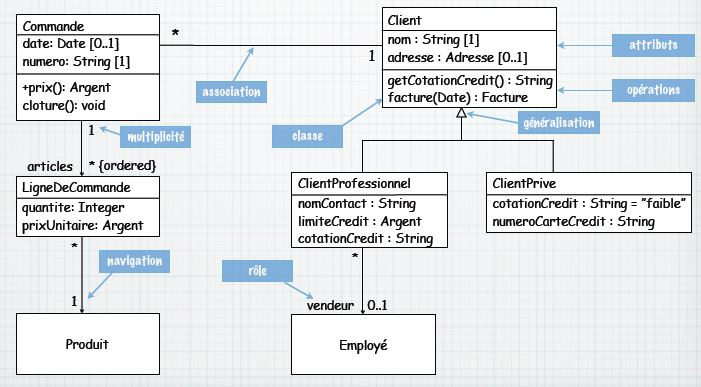
\includegraphics[scale=0.8]{diagramme_classes.jpg}
  \caption{Exemple d'un diagramme de classes UML}
  \label{diagramme_classes}
\end{figure}

\hspace*{-.75cm}Les différentes multiplicités possibles sont les suivantes :
\begin{description}
  \item[$m$] doit avoir exactement $m$ (peut valoir *).
  \item[$m$..$n$] peut avoir entre $m$ et $n$.
  \item[$m$..*] minimum $m$.
\end{description}
Les différents modes de visibilité sont les suivants :
\begin{description}
  \item[+]	Public, ouvert aux autres classes
  \item[\#]	Protégé, uniquement visible par les sous-classes
  \item[$-$]	Privé, uniquement accessible par cette classe
\end{description}
Des \strong{contraintes} sur les attributs sont notés entre accolades.
Des \strong{notes} peuvent être ajoutées au diagramme pour le clarifier.
Une note se manifeste par une boîte repliée qui est
reliée en pointillé à la boîte qu'elle clarifie.
On explicite aussi les \strong{attributs dérivés} par la présence
d'un / avant le nom de l'attribut.
Un attribut est dérivé si sa valeur peut être retrouvée
grâce à d'autres attributs.
La figure~\ref{diagramme_classes_addon} illustre
comment représenter un attribut dérivé et sa contrainte dans une note associée.
\begin{figure}[h]
  \centering
  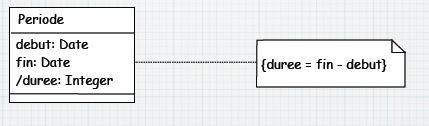
\includegraphics[scale=1]{diagramme_classes_addon.jpg}
  \caption{Représentation d'un attribut dérivé, d'une contrainte et d'une note}
  \label{diagramme_classes_addon}
\end{figure}

Pour exprimer une \strong{association binaire},
on relie simplement les deux classes concernées.
On utilise en fait les associations lorsqu'un attribut n'est pas de type primitif.
Ainsi si on veut exprimer le fait qu'un client a des commandes (objet),
on le relie à la classe Commande.

Sur la ligne d'association,
on retrouve diverses informations tel qu'un nom (plus sens de lecture),
deux rôles (un a chaque extrémité) et les multiplicités associées aux classes.

Si l'association n'est pas à double sens
(c'est à dire si la classe A peut accéder à B mais pas l'inverse),
alors on placera une flèche (plutôt qu'une ligne) allant de A vers B.
On dit alors que c'est une \strong{navigation}.

La figure~\ref{diagramme_classes_association}
représente une exemple d'association binaire.
\begin{figure}[h]
  \centering
  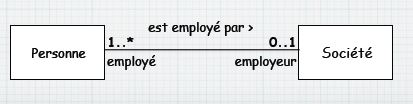
\includegraphics[scale=1]{diagramme_classes_association.jpg}
  \caption{Exemple d'une association binaire entre employé et employeur}
  \label{diagramme_classes_association}
\end{figure}

Une \strong{généralisation} exprime que certaines classes
``dérivent'' d'une classe mère,
est une sorte de...
En java, on dit qu'une classe hérite d'une autre.
Cela se représente par une flèche ouverte.
Cela peut être nécessaire notamment dans le cas d'une
\strong{classe abstraite} non instanciée mais qui
est présente pour clarifier les choses.
La figure~\ref{diagramme_classes_generalisation} représente ces deux concepts
\begin{figure}[h]
  \centering
  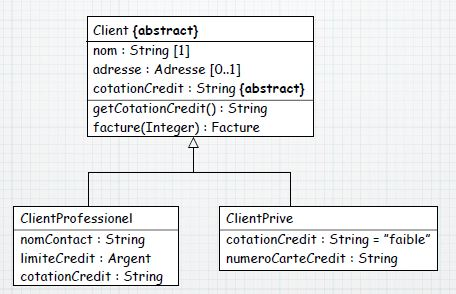
\includegraphics[scale=0.8]{diagramme_classes_generalisation}
  \caption{Exemple d'une généralisation et d'une classe abstraite}
  \label{diagramme_classes_generalisation}
\end{figure}

Il existe encore d'autres relations aux notations particulières.
Celles-ci sont reprises sur la figure~\ref{diagramme_classes_relations}.

On peut retrouver des \strong{dépendances}.
Représenté par une flèche en pointillé,
elle est ornée d'un mot-clé qui décrit la relation
d'utilisation entre la source et la cible.
On distingue
\begin{description}
  \item[call]
    la classe source appelle une opération dans la classe cible,
  \item[create]
    la classe source crée une instance de la classe cible,
  \item[use]
    la classe source a besoin de la classe cible pour son implémentation.
\end{description}

\begin{figure}[h]
  \centering
  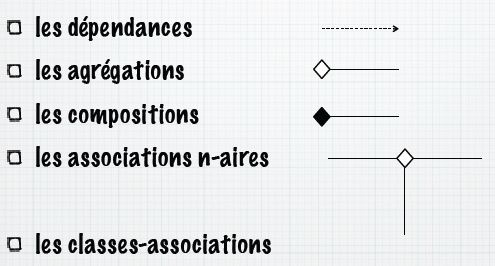
\includegraphics[scale=0.6]{diagramme_classes_relations}
  \caption{Notations des autres relations}
  \label{diagramme_classes_relations}
\end{figure}

L'\strong{agrégation} représente une association non symétrique dans laquelle
une des extrémités joue un rôle prédominant par rapport à l'autre extrémité.
La différence avec l'association est floue et on ne l'utilisera donc pas.

La \strong{composition} décrit une relation de contenance
physique (exemple : un polygone contient des points).
Pour savoir si c'est un composition, on regarde si lorsqu'on supprime
un élément d'une base de donnée, l'autre doit être supprimé également.
Par exemple, si on supprime un restaurant, il faut aussi supprimer
ses plages horaires.
Mais si on supprime un utilisateurs, il ne faut pas supprimer ses amis.

L'\strong{association $n$-aire} relie plus de deux classes entre elles.
Généralement le lieu de rencontre peut être remplacé par une nouvelle
classe que l'on nomme \strong{classe-association}.
Par exemple,
l'association Etudiant-Enseignant-Salle peut donné lieu à la classe Cours.

Lors de la réalisation d'un diagramme de classe UML,
il est important de penser orienté objet,
et de bien penser à toutes les responsabilités,
opérations qu'une classe doit pouvoir effectuer.

\section{Le diagramme de séquence UML}
Dernière étape du processus de développement,
le \strong{diagramme de séquence UML} permet de penser
la \emph{structure dynamique} de l'application.
Rappelons en effet que le diagramme de classes traitait
de la \emph{structure statique} de l'application.
Contrairement au diagramme de classes qui se basait sur les cartes CRC,
le diagramme de séquences se base sur les histoires
utilisateurs pour se structurer.
Typiquement, un diagramme de séquence décrit le comportement d'un
seul scénario et ne regroupera donc qu'une ou quelques histoires utilisateurs.
Sur l'axe horizontal,
on retrouvera les objets \emph{participants} et sur
l'axe vertical la chronologie des événements.
Un diagramme est constitué de \emph{messages} et
est toujours initialisé par un \emph{message trouvé}.
La figure~\ref{diagramme_sequences} montre un
exemple de diagramme avec ses différents composants.

\begin{figure}[h]
  \centering
  \hspace*{-0.25cm}
  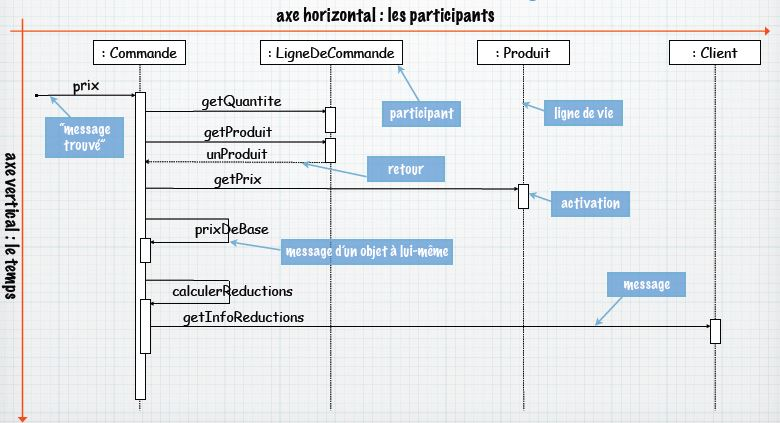
\includegraphics[scale=0.75]{diagramme_sequences.jpg}
  \caption{Composants d'un diagramme de séquences}
  \label{diagramme_sequences}
\end{figure}

Chaque participant est représenté par une ``boîte de ligne de vie''.
Une collection d'un type de participants sera représenté par une double boîte.
Des messages, représenté par des flèches,
partent de cette ligne de vie et ont la syntaxe suivante
\begin{verbatim}
retour = message(paramètre : typeParamètre) : typeRetour
\end{verbatim}
Le message est essentiel et les autres informations peuvent être omises.
Un message particulier est celui qui initiale le diagramme:
le message trouvé; il est représenté par un cercle noir.
Une ligne de vie possède une ou plusieurs barre d'activation
indiquant quand un participant est actif dans une interaction.
À un message correspond une réponse ou retour qui a la syntaxe:
\begin{verbatim}
valeurDeRetour = message(paramètre)
\end{verbatim}
Cette syntaxe fait deux choses en même temps : le message et le retour.
On peut expliciter les deux en faisant deux étapes:
le message comme décrit ci-dessus et le retour que l'on présentera
par une flèche en pointillé sur laquelle on écrit la valeur de retour.
Un objet peut également s'envoyer un message à lui-même.

Le diagramme de séquence permet aussi la création et la destruction d'objets.
La manière de procéder est illustré
par la figure~\ref{diagramme_sequences_objet}.
\begin{figure}[h]
  \centering
  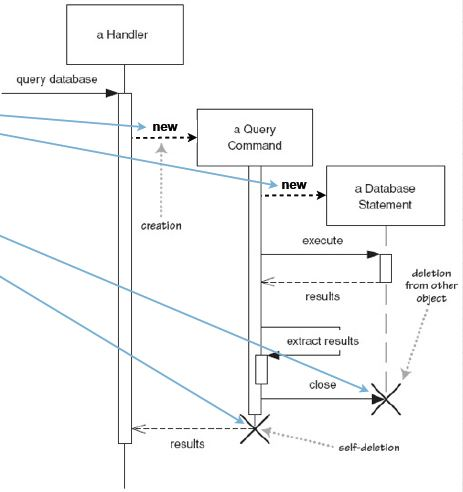
\includegraphics[scale=0.75]{diagramme_sequences_objet.jpg}
  \caption{Création et destruction d'objets dans un diagramme de séquences}
  \label{diagramme_sequences_objet}
\end{figure}

Pour terminer,
il faut pouvoir modéliser les structures conditionnelles et itératives.
Pour cela,
UML utilise des cadres (voir figure~\ref{diagramme_sequences_cadres}).
Un cadre est muni d'un \emph{opérateur} et d'une \emph{garde}.
\begin{figure}[h]
  \centering
  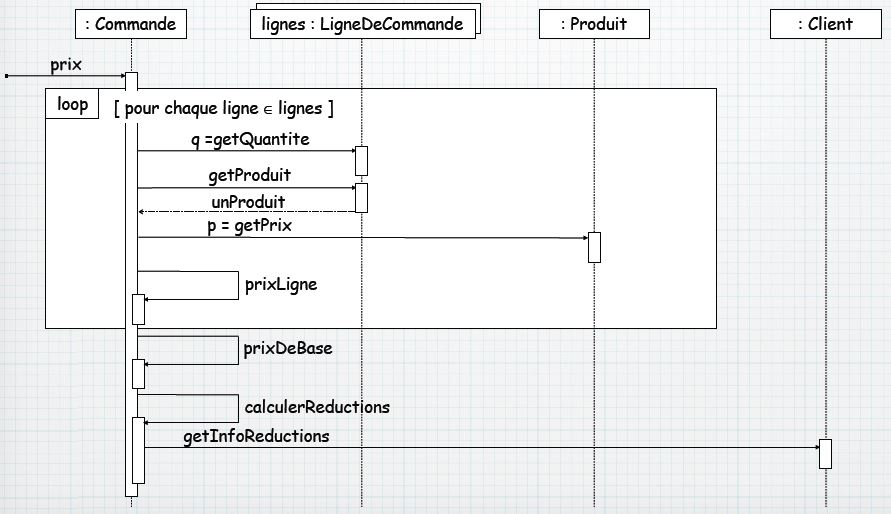
\includegraphics[scale=0.60]{diagramme_sequences_cadres.jpg}
  \caption{Exemple d'un cadre itératif dans un diagramme de séquence}
  \label{diagramme_sequences_cadres}
\end{figure}
Les trois opérateurs usuels sont les suivants
\begin{description}
  \item[alt] représente la condition if-else où le else est
    une garde séparé du if par des pointillé.
  \item[loop] représente la boucle for
  \item[opt] représente le condition if
\end{description}

\end{document}
